\section{Experiment Details}
\label{sec:experiment_details}

\subsection{Model Configurations and Hyperparameters}

We summarize the details required to replicate our experiments below.

\subsubsection{Image Classification}

\textbf{Baseline Model:} For dense models, we use standard implementations of
ViT~\citep{dosovitskiy2020image}, MLP-Mixer{tolstikhin2021mlp} from the
\texttt{timm} library and from the T2T-ViT codebase~\citep{yuan2021tokens}.

The Monarch version of these models simply swap out the dense weight matrices in the attention blocks (projection matrices) and in the FFN block (linear layers) with Monarch matrices.
We set the number of blocks in the block-diagonal matrices to 4.
We also reduce the amount of regularization (stochastic depth) as our Monarch models are smaller than the dense models.

We adopt the hyperparameters (optimizer, learning rate, learning rate
scheduler) from~\citet{yuan2021tokens}.
Details are in~\cref{table:imagenet_hparams}.

We measure the wall-clock training time on V100 GPUs.

\begin{table}[!htbp]
 \caption{Configuration of the ImageNet experiment}   
\centering
\resizebox{0.8\linewidth}{!}{
\noindent\begin{tabular}{@{}c||ccccccc@{}}
  \specialrule{.15em}{.05em}{.05em}
Model&\multicolumn{1}{c}{Optimizer}&\multicolumn{1}{c}{Weight Decay}&\multicolumn{1}{c}{Learning Rate}&\multicolumn{1}{c}{Drop Path}&\multicolumn{1}{c}{Warmup/Epoch}\\
  \specialrule{.15em}{.05em}{.05em}
ViT-Small& AdamW & 0.05 & 0.001 & 0.1& 5/300 \\
Monarch-ViT-Small& AdamW & 0.05 & 0.001 &0& 5/300 \\
ViT-Base& AdamW & 0.05 & 0.001 &0.1& 5/300 \\
Monarch-ViT-Base& AdamW & 0.05 & 0.001 &0& 5/300 \\
  \specialrule{.15em}{.05em}{.05em}
Mixer-Small &AdamW& 0.1 &0.001&0.1& 5/300 \\
Monarch-Mixer-Small &AdamW&0.1 &0.001& 0 & 5/300 \\
Mixer-Base &AdamW& 0.1 &0.001&0.1& 5/300 \\
Monarch-Mixer-Base &AdamW &0.1 &0.001& 0 & 5/300 \\
  \specialrule{.15em}{.05em}{.05em}
\end{tabular}
}
\label{table:imagenet_hparams}
\end{table}

We follow the naming convention in the Vision Transformer paper and MLP-Mixer paper. In particular, ViT-S and ViT-B refers to the small and base ViT models respectively, and 16 refers to the patch size of 16x16. The MLP-Mixer models follow the same convention.

\subsubsection{Language Modeling}
For dense models, we use standard implementations of
GPT-2~\citep{radford2019language} from Huggingface \texttt{transformers} library and from Nvidia's Megatron-LM repo. 
We follow the training recipe of the Megatron-LM repo.

The Monarch version of these models simply swap out the dense weight matrices in the attention blocks (projection matrices) and in the FFN block (linear layers) with Monarch matrices.
We set the number of blocks in the block-diagonal matrices to 4.
We also reduce the regularization strength (dropout) as our model is smaller.

We report the hyperparameters used in~\cref{table:wt103} and~\cref{table:owt}.
We use an effective batch size of 512, and use gradient accumulation to fit into available GPU memory.

We measure the wall-clock training time on V100 GPUs.
\begin{table}[!h]
    \vspace{-0.5cm}
\centering
\caption{Configuration of the WikiText-103 experiments}
\resizebox{0.8\linewidth}{!}{
\noindent\begin{tabular}{@{}c||ccccccc@{}}
  \specialrule{.15em}{.05em}{.05em}
Model&\multicolumn{1}{c}{Optimizer}&\multicolumn{1}{c}{Weight Decay}&\multicolumn{1}{c}{Learning Rate}&\multicolumn{1}{c}{Dropout}&\multicolumn{1}{c}{Warmup/Epoch}\\
  \specialrule{.15em}{.05em}{.05em}
GPT-2-small& AdamW & 0.1 & 6e-4 & 0.1& 10/100 \\
Monarch-GPT-2-small& AdamW & 0.1 & 6e-4 & 0.0 & 10/100 \\
GPT-2-medium& AdamW & 0.1 & 1.5e-4 & 0.1& 10/100 \\
Monarch-GPT-2-medium & AdamW & 0.1 & 1.5e-4 & 0.0 & 10/100 \\
  \specialrule{.15em}{.05em}{.05em}
\end{tabular}
}
\label{table:wt103}
\end{table}

\begin{table}[!h]
\vspace{-0.5cm}
\centering
\caption{Configuration of the OpenWebText experiments}
\resizebox{0.8\linewidth}{!}{
\noindent\begin{tabular}{@{}c||ccccccc@{}}
  \specialrule{.15em}{.05em}{.05em}
Model&\multicolumn{1}{c}{Optimizer}&\multicolumn{1}{c}{Weight Decay}&\multicolumn{1}{c}{Learning Rate}&\multicolumn{1}{c}{Dropout}&\multicolumn{1}{c}{Warmup/Total iterations}\\
  \specialrule{.15em}{.05em}{.05em}
GPT-2-Small& AdamW & 0.1 & 6e-4 & 0.1& 4k/400k \\
Monarch-GPT-2-Small & AdamW & 0.1 & 6e-4 & 0.0 & 4k/400k \\
GPT-2-Medium& AdamW & 0.1 & 1.5e-4 & 0.1& 4k/400k \\
Monarch-GPT-2-Medium & AdamW & 0.1 & 1.5e-4 & 0.0 & 4k/400k \\
  \specialrule{.15em}{.05em}{.05em}
\end{tabular}
}
\label{table:owt}
\end{table}


\subsection{Details for PDE Solving}
We adopt the experiment setting and data generation of Navier-Stokes Equation from FNO~\citep{li2020fourier}. It considers the 2-d Navier-Stokes equation for a viscous, incompressible fliud in vorticity form on the unit tortus:
\begin{align}
    \partial_{t} w(x, t) + u(x, t) \cdot \nabla w(x, t) & = v \Delta w(x, t) + f(x), & x \in (0, 1)^2, t \in (0, T] \\
    \nabla w(x, t) & = 0, & x \in (0, 1)^2, t \in (0, T] \\
    w(x, 0) & = w_0(x), & x \in (0, 1)^2 \\
\end{align}
where $u \in C([, T0])$;$H_{per}((0, 1)^2; \mathbb{R}^2))$ for any $r>0$ is the velocity field, $w=\nabla \times u$ is the vorticity, $w_0 \in L^2_{per}((0, 1)^2; \mathbb{R})$ is the initial vorticity, $v \in \mathbb{R_{+}}$ is the viscosity coefficient, and $f \in L_{per}^2((0, 1)^2; \mathbb{R})$ is the forcing function. 
$T$ represents the time interval since it is time-dependent equation. $v$ represents the viscosity. N represents the number of training pairs or data. \cref{table:pde} shows the results for viscosities $v=1e-3, 1e-4, 1e-5$, $T=50, 30, 20$ respectively and use $N=1000$. 

\subsection{Details for GPT-2 Downstream Tasks}
We train Pixelfly-GPT2-small on a larger scale dataset, OpenWebText, and evaluate the downstream quality on zero-shot generation and classification tasks from~\citep{zhao2021calibrate}, achieving comparable and even better performance to the dense model. Specifically, the datasets contains five popular classification tasks: SST2, Trec, CB, Agnews, and Dbpedia. We also adapated the calibrated metric from~\citep{zhao2021calibrate} for evaluation. Results for each individual task are shown in~\cref{table:gpt_finetune_full}. 

\begin{table}[h]
  \small
  \centering
  \vspace{-3mm}
  \caption{\label{table:gpt_finetune_full}The performance (accuracy) of GPT-2-medium trained with Monarch reverse sparsification and with conventional dense training on text classification benchmarks.}
  \setlength{\tabcolsep}{5pt}
  \vspace{1em}
   \resizebox{0.7\linewidth}{!}{
  \begin{tabular}{@{}c||ccccc@{}}
    \specialrule{.15em}{.05em}{.05em}
    Model&\multicolumn{1}{c}{OpenWebText (ppl)}&\multicolumn{1}{c}{Speedup}& \multicolumn{1}{c}{Classification (avg acc)} \\
    \specialrule{.15em}{.05em}{.05em}
    GPT-2m& 68.3 & 37.0 & 10.7 & 52.0 & 26.6\\
    Monarch-GPT-2m& 72 & 38.6 & 12.5 & 47.3 & 23.0 \\
    \specialrule{.15em}{.05em}{.05em}
  \end{tabular}
  }
  \vspace{-3mm}
\end{table}

\subsection{Details for BERT Pretraining}
\label{subsec:bert_details}

We follow the training procedure and hyperparameters of the reference
implementation from Nvidia Deep Learning examples
(\url{https://github.com/NVIDIA/DeepLearningExamples}).
In particular, we use the LAMB optimizer with learning rate 4e-3.
We use as large a minibatch size as possible that still fits in the GPU memory
(A100-40GB), and use gradient accumulation to reach an effective batch size of
64k sequences for phase 1 (maximum sequence length 128) and 32k for phase 2
(maximum sequence legnth 512).
We train is mixed precision (fp16 and fp32).

We use all the optimizations that were in Nvidia's BERT implementation
in MLPerf 1.1:
\begin{enumerate}
  \item Only compute the prediction scores (last layer) for masked tokens as
  the outputs of other tokens are not used to compute the masked language
  modeling loss.
  \item Remove padding tokens and only compute the attention for non-padding
  tokens.
  \item Use a fused CUDA kernel (FMHA) that combines 4 steps into one kernel: computes
  $Q K^T$, take softmax, apply dropout, multiply by $V$, where $Q, K, V$ are the
  query, key, and value respectively.
  \item Fuse matrix multiplication and adding bias into one CUDA kernel in the feed-forward network
  (FFN) layers. The gradient of the bias is also fused with the matrix
  multiplication the backward pass.
  \item Fuse matrix multiplication and adding bias into one CUDA kernel in the
  attention output projection.
  \item Fuse dropout and adding residual in the residual connection at the end
  on the attention and FFN blocks.
\end{enumerate}

We train with DeepSpeed~\citep{rasley2020deepspeed} ZeRO optimizer stage 1 to
shard the optimizer states, thus reducing GPU memory usage and allowing us to
use larger batch sizes.
For the Nvidia MLPerf implementation, we report the speed for both Apex's
automatic mix-precision (AMP) level O2 (as in the original implementation), and
DeepSpeed ZeRO optimizer.

\subsection{Accelerated Multi-coil MRI Reconstruction}
\label{sec:experiment_details_mri}

\subsubsection{Background}
In multi-coil MRI, multiple receiver coils (i.e. sensors) acquire complex-valued measurements in the spatial frequency (a.k.a. \textit{k-space}) domain. These measurements are modulated by the spatially-varying sensitivity maps, which characterize the sensitivity of each coil to the imaging target. In accelerated MRI, scan times are reduced by decreasing the number of samples acquired in k-space. Because the data is sampled below the Nyquist rate, reconstructing the underlying image is an ill-posed problem.

The forward problem for accelerated multi-coil MRI can be written as the matrix equation
\begin{equation*}
    y = \Omega\boldsymbol{F}\boldsymbol{S}x + \epsilon
\end{equation*}
where $\Omega$ is the binary undersampling mask that indexes acquired samples in k-space, $y$ is the vectorized measured signal in k-space, $\boldsymbol{F}$ is the discrete Fourier transform matrix, $\boldsymbol{S}$ is the receiver coil sensitivity maps,  $x$ is the ground-truth signal in image-space, and $\epsilon$ is additive complex Gaussian noise. The acceleration factor is given by $R = \frac{\sum_i^{|N|} \Omega_i}{|\Omega|}$.

\subsubsection{Experimental Details}

\paragraph{Dataset.} We benchmark our method on the SKM-TEA Raw Data Track, which consists of dual-echo 3D MRI scans \citep{desai2021skm}. Scans are accelerated using Poisson Disc undersampling masks distributed with the dataset. During training, Poisson Disc masks are generated, cached, and applied to mask the k-space data to simulate accelerated scans.

\paragraph{Matrix Shape.} Like all matrices, Monarch matrices have an explicit shape constraint, which is a limitation of these matrices for MRI reconstruction tasks. Thus, the SKM-TEA dataset was filtered to include scans of shape $512 \times 512 \times 160$, which is the most frequently occuring scan shape. A total of 3 scans were dropped from the original 155 scans in the dataset. Our method and all baselines were trained on this filtered dataset.

\begin{table}[!ht]
    \vspace{-0.5cm}
\centering
\caption{Baseline configurations of the SKM-TEA MRI reconstruction experiments.}
\resizebox{0.6\linewidth}{!}{
\noindent\begin{tabular}{c||cccccc}
  \specialrule{.15em}{.05em}{.05em}
Model & Params & Optimizer & Weight Decay & Learning Rate & Epoch \\
  \specialrule{.15em}{.05em}{.05em}
SENSE & --- & --- & --- & --- & --- \\
U-Net &  7.8M & Adam & 1e-4 & 1e-3 & 20 \\
mSENSE  & 57.5K & Adam & 1e-4 & 1e-3 & 20 \\
  \specialrule{.15em}{.05em}{.05em}
\end{tabular}
}
\label{table:skmtea-config}
\end{table}


\paragraph{Baselines.} We compare our method to two baselines, SENSE and U-Net. Parameter count and hyperparameters are available in Table \ref{table:skmtea-config}.
\begin{itemize}
    \item \textit{SENSE}: SENSE performs a linear combination of the images acquired on each coil \citep{pruessmann1999sense}. Here, the inverse fsat Fourier transform (IFFT) is applied to the acquired k-space for each coil. The resulting images are combined into a single complex image by weighting each coil image by corresponding coil sensitivity maps. In accelerated MRI, the unsampled frequencies are zero-valued; thus, SENSE produces a \textit{zero-filled image}. Note, SENSE does not require any training.
    \item \textit{U-Net}: U-Net is a popular fully convolutional neural network baseline for MRI reconstruction \citep{ronneberger2015u}. We use the default implementation and hyperparameters used by \citet{desai2021skm} to benchmark the SKM-TEA dataset. In this approach, the SENSE-reconstructed zero-filled image is mapped to SENSE-reconstructed ground truth images.
\end{itemize}

\paragraph{Monarch-SENSE (mSENSE):} We propose a modification to the SENSE method, in which the (IFFT) is parameterized by a factorized Monarch matrix. This matrix is initialized to the IFFT but, unlike SENSE, is learnable. While mSENSE is trainable, it has 137x fewer trainable parameters than U-Net.

\paragraph{Metrics:} We evaluate reconstruction performance using peak signal-to-noise ratio (pSNR) and structural similarity (SSIM) on both echoes (echo1 - E1, echo2 - E2) separately. Both metrics were computed on the 3D volume of each echo.

\paragraph{Extended Results.} We provide sample reconstructions of SENSE, mSENSE, and U-Net in data-limited settings for first (Fig.~\ref{fig:mri-data-limited-echo1}) and second (Fig.~\ref{fig:mri-data-limited-echo2}) echoes. Both SENSE and U-Net reconstructed images have aliasing artifacts. Due to the random Poisson Disc undersampling pattern, these artifacts are incoherent, causing them to manifest as blurring around fine structures and edges. In contrast, mSENSE can recover these structures with higher fidelity. Even in the second echo, which has lower signal-to-noise ratio (SNR) than the first echo, mSENSE does not overblur the image.

\begin{figure}
    \centering
    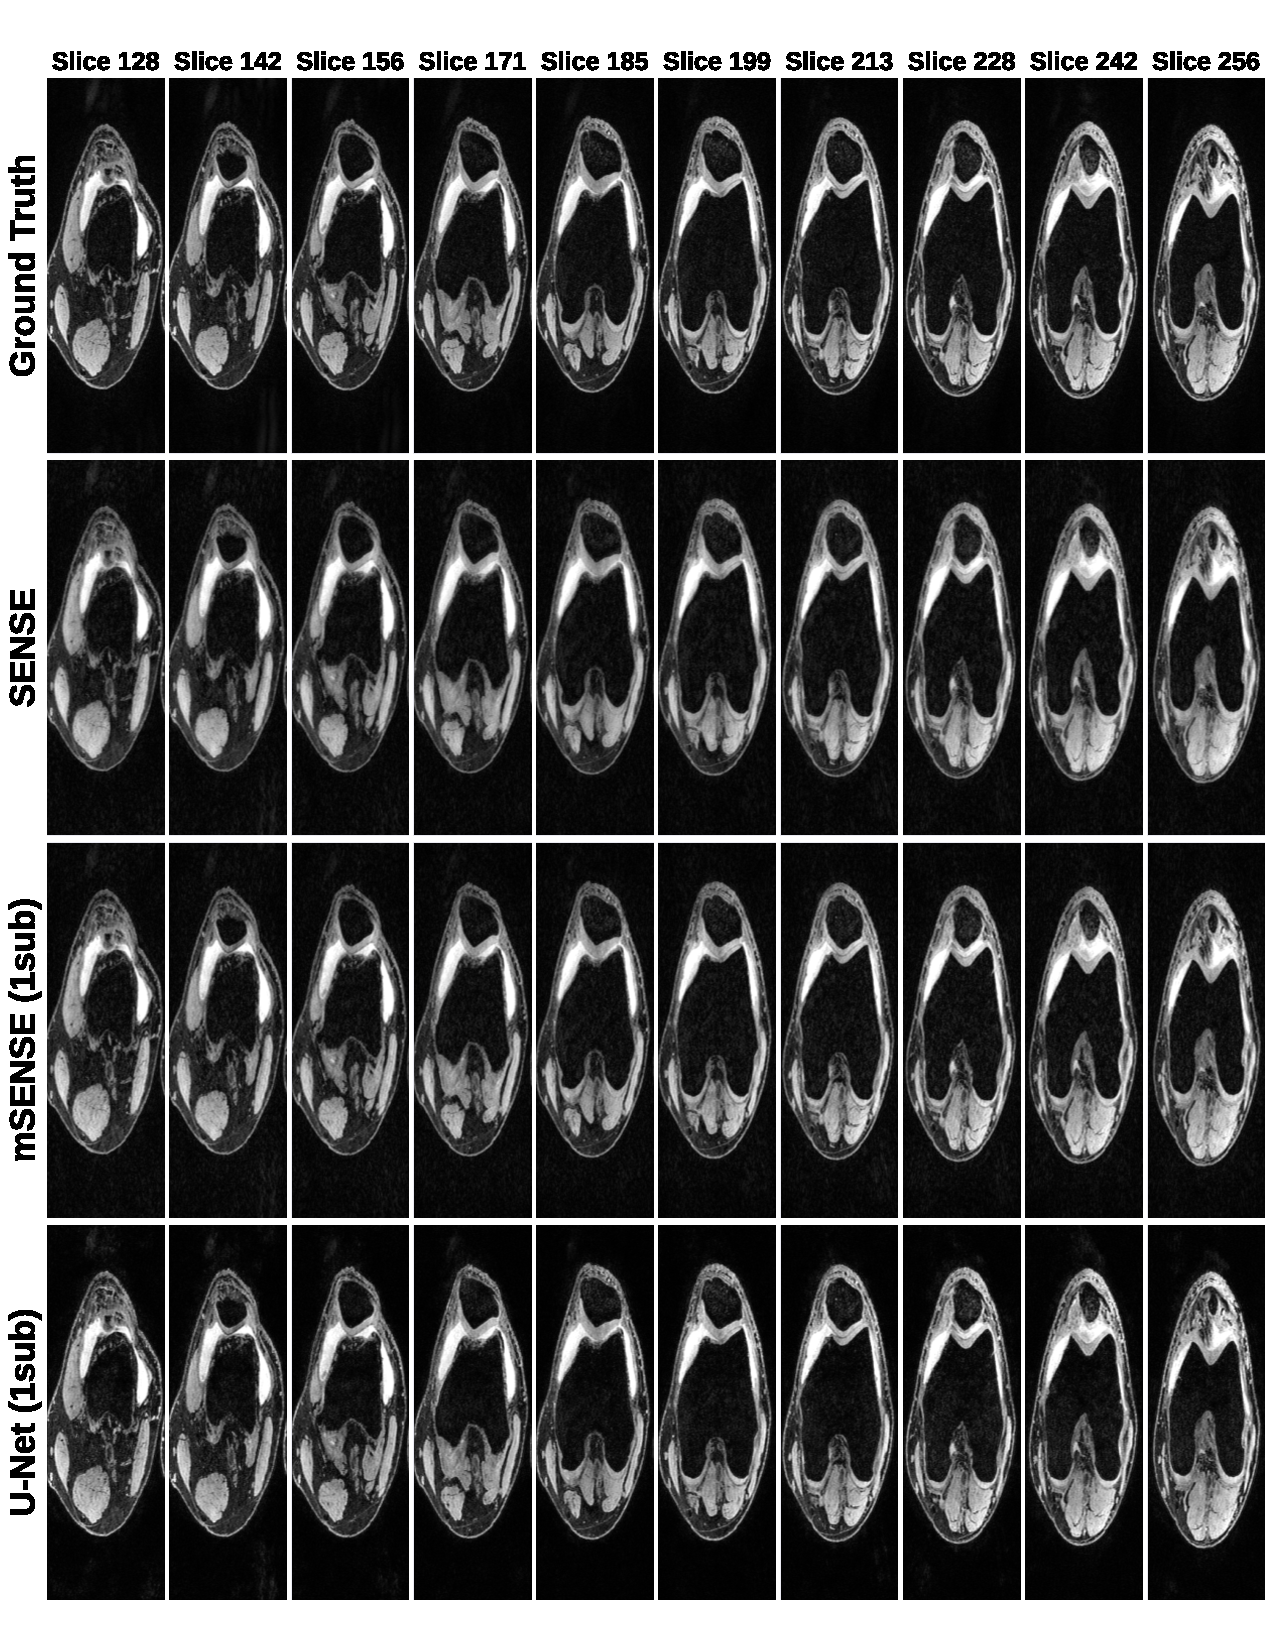
\includegraphics[width=0.9\linewidth]{figures/sample-mri-echo1.pdf}
    \vspace{-1em}
    \caption{Sample reconstructions at 2x acceleration for the first echo in the SKM-TEA dataset using SENSE, Monarch-SENSE (mSENSE), and U-Net. Both mSENSE and U-Net are trained with 1 training scan. SENSE is an untrained method.}
    \label{fig:mri-data-limited-echo1}
\end{figure}

\begin{figure}
    \centering
    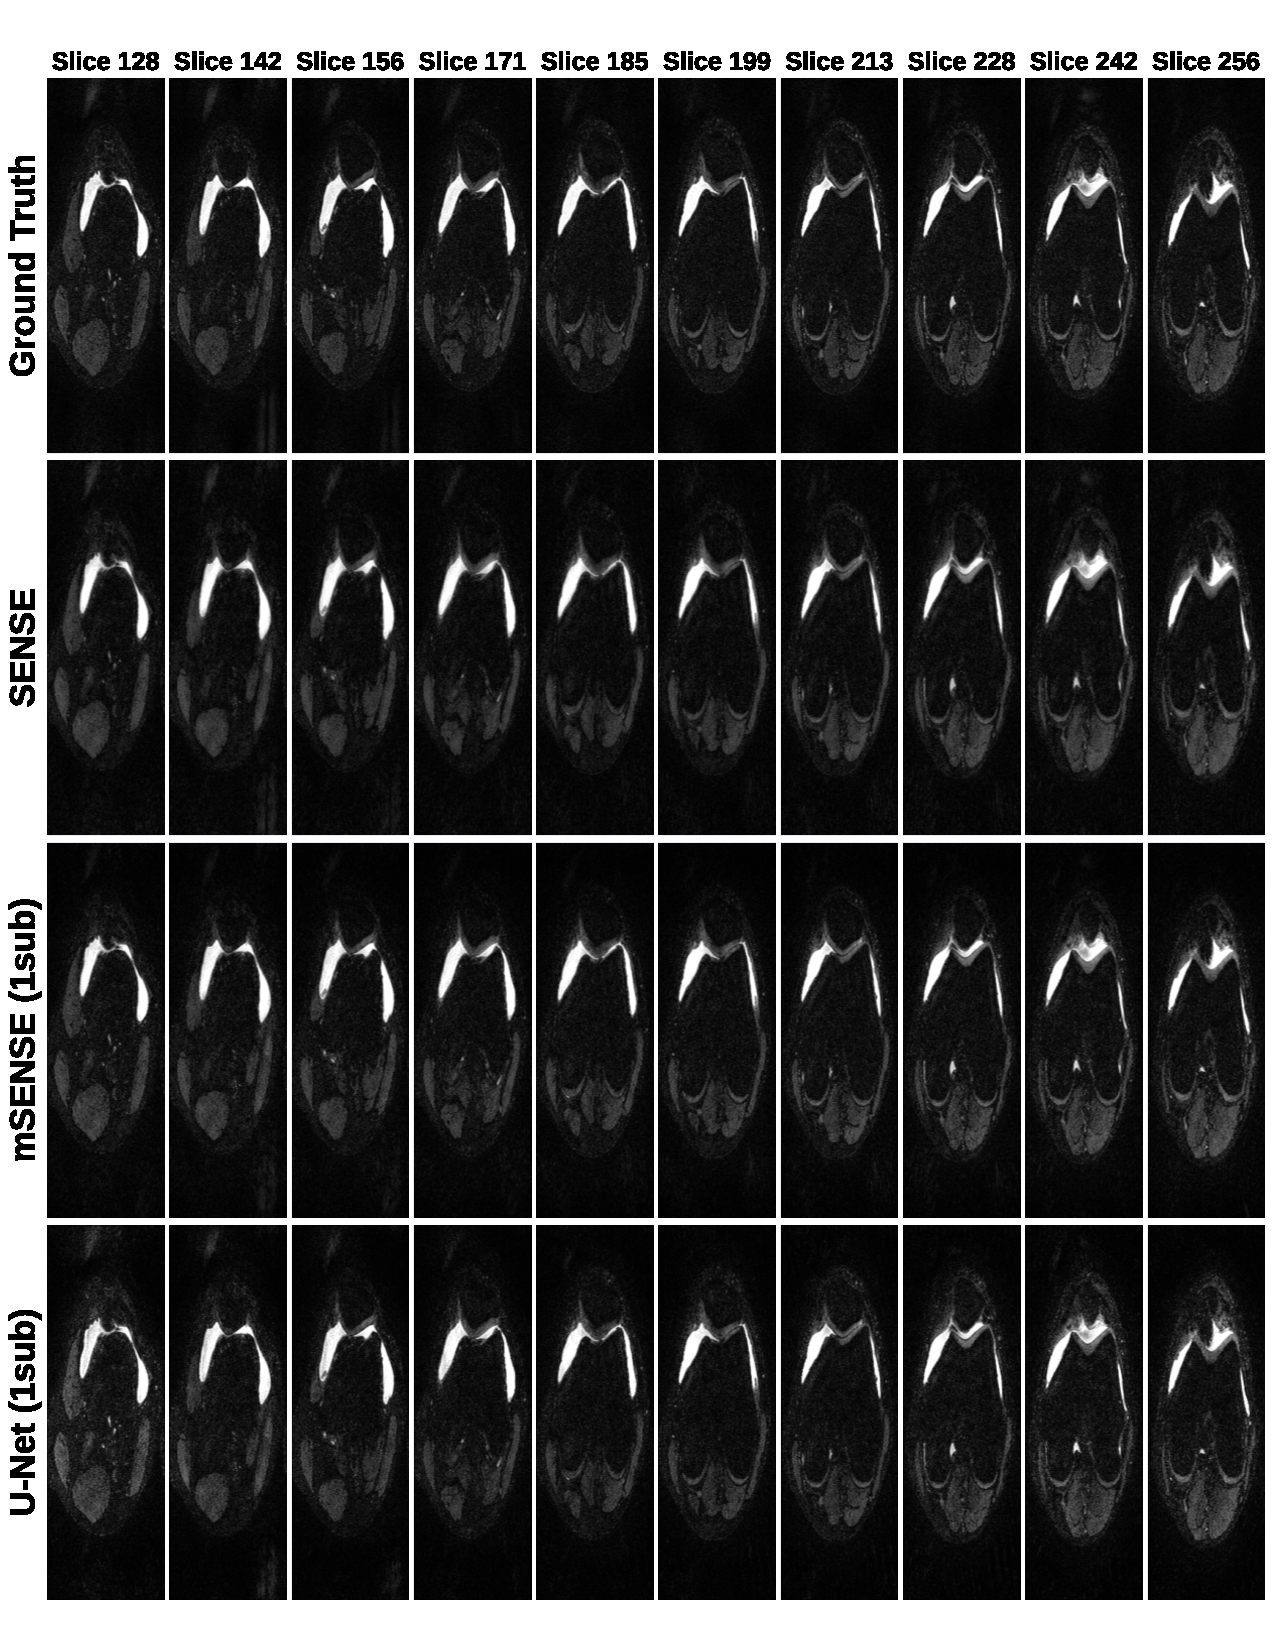
\includegraphics[width=6in]{figures/sample-mri-echo2.pdf}
    \vspace{-1em}
    \caption{Sample reconstructions at 2x acceleration for the second echo in the SKM-TEA dataset using SENSE, Monarch SENSE (mSENSE), and U-Net. Both mSENSE and U-Net are trained with 1 training scan. SENSE is an untrained method.}
    \label{fig:mri-data-limited-echo2}
\end{figure}






